\documentclass{article}

\usepackage{geometry}
\usepackage{amsmath}
\usepackage{graphicx}
\usepackage{listings}
\usepackage{hyperref}
\usepackage{multicol}
\usepackage{fancyhdr}
\pagestyle{fancy}
\hypersetup{ colorlinks=true, linkcolor=black, filecolor=magenta, urlcolor=cyan}
\geometry{ a4paper, total={170mm,257mm}, top=20mm, right=20mm, bottom=20mm, left=20mm}
\setlength{\parindent}{0pt}
\setlength{\parskip}{1em}
\renewcommand{\headrulewidth}{0pt}
\lhead{Competitive Programming - Arkavidia V}
\fancyfoot[CE,CO]{\thepage}
\lstset{
    basicstyle=\ttfamily\small,
    columns=fixed,
    extendedchars=true,
    breaklines=true,
    tabsize=2,
    prebreak=\raisebox{0ex}[0ex][0ex]{\ensuremath{\hookleftarrow}},
    frame=none,
    showtabs=false,
    showspaces=false,
    showstringspaces=false,
    prebreak={},
    keywordstyle=\color[rgb]{0.627,0.126,0.941},
    commentstyle=\color[rgb]{0.133,0.545,0.133},
    stringstyle=\color[rgb]{01,0,0},
    captionpos=t,
    escapeinside={(\%}{\%)}
}


\begin{document}

\begin{center}
    \section*{A. Arvy Menjemur Pakaian}

    \begin{tabular}{ | c c | }
        \hline
        Batas Waktu  & 1s \\
        Batas Memori & 512MB \\
        \hline
    \end{tabular}
\end{center}

\subsection*{Deskripsi}

Saat berjualan pakaian, terjadi kecelakaan sehingga $M$ potong baju menjadi kotor.
Daripada terbuang sia-sia, Arvy memutuskan untuk mencuci baju kotor tersebut dan menggunakannya sendiri.

Setelah dicuci, ia menjemur menggunakan jemuran berbentuk gurita.
Lalu, ia terpikir sebuah teka-teki.

\begin{center}
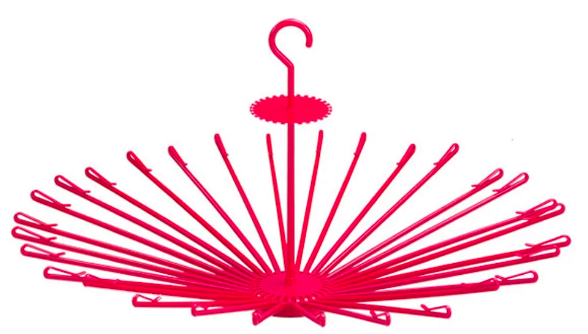
\includegraphics[width=200px]{jemuran}

\footnotesize Sumber: \href{https://www.bukalapak.com/p/perlengkapan-bayi/perlengkapan-bayi-lainnya/9plhup-jual-jemuran-gantungan-baju-pakaian-bayi-lion-star-folding-hanger-30-sticks-besar-jemuran-gurita}{bukalapak.com}
\end{center}

Jika ia memiliki sebuah jemuran gurita dengan $N$ tangan (artinya, ada $N$ tempat menggantungkan pakaian), apakah ada konfigurasi untuk menjemur $M$ pakaian yang tidak membuat jemuran berat sebelah? Anda dapat mengasumsikan antar tangan jemuran memiliki jarak yang sama, semua pakaian memiliki berat yang sama, dan dijemur pada jarak yang sama dari titik pusat.

Sebuah konfigurasi dianggap tidak membuat jemuran berat sebelah jika resultan dari gaya berat pakaian hanya mengarah ke bawah (tidak ada gaya arah horizontal).

\subsection*{Format Masukan}
Baris pertama terdiri dari satu bilangan bulat positif $T$ ($1 \leq T \leq 100$), menyatakan banyaknya kasus uji.
Tiap kasus uji terdiri dari bilangan $N$ dan $M$ ($1 \leq M \leq N \leq 200.000$) menyatakan banyaknya tangan gurita dan banyaknya pakaian.

\subsection*{Format Keluaran}
Untuk tiap kasus uji, keluarkan \lstinline{YA} jika ada konfigurasi yang diminta, atau \lstinline{NO} jika tidak.

\begin{multicols}{2}
\subsection*{Contoh Masukan}
\begin{lstlisting}
4
4 2
10 4
10 1
12 7
\end{lstlisting}
\columnbreak
\subsection*{Contoh Keluaran}
\begin{lstlisting}
YA
YA
TIDAK
YA
\end{lstlisting}
\vfill
\null
\end{multicols}

\pagebreak

\subsection*{Penjelasan}
Pada kasus uji pertama, konfigurasi yang mungkin salah satu dengan menaruh pakaian di titik berwarna merah:

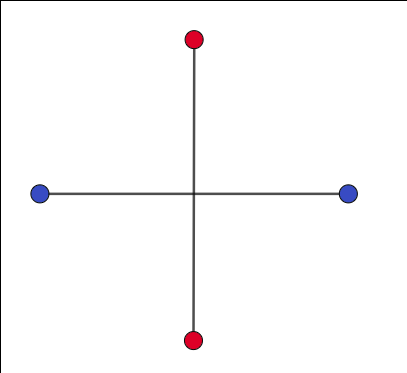
\includegraphics[width=200px]{sample-1}

Pada kasus uji kedua, konfigurasi yang mungkin salah satu dengan menaruh pakaian di titik berwarna merah:

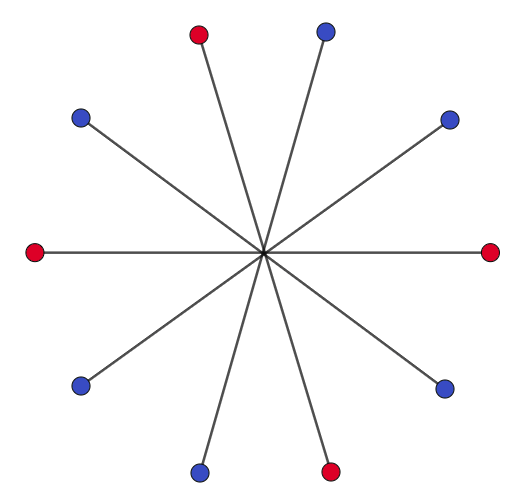
\includegraphics[width=200px]{sample-2}

Pada kasus uji keempat, konfigurasi yang mungkin salah satu dengan menaruh pakaian di titik berwarna merah:

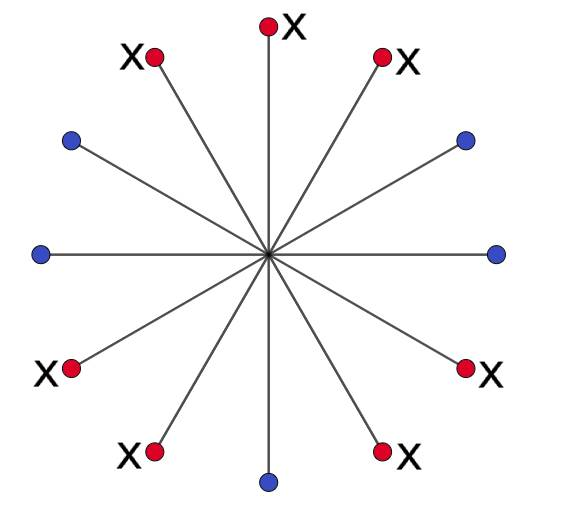
\includegraphics[width=200px]{sample-4}

\end{document}